\section{HMC for a spin--fermion model}
\renewcommand{\currentEdge}{stats-physics}

\begin{frame}{Statistics + Physics}
  \begin{center}
    \ResearchTriangle{stats-physics}
  \end{center}
\end{frame}

\begin{frame}{Sampling is the shared bottleneck}
  \begin{columns}[T]
    \begin{column}{0.32\textwidth}
      \textbf{Bayes}
      \[
        p(\theta\mid y)
        =
        \frac{p(y\mid\theta)\,p(\theta)}{p(y)}
      \]
      {\small Need samples from the posterior when $p(y)$ is intractable.}
    \end{column}
    \begin{column}{0.32\textwidth}
      \textbf{Stat.~mech.}
      \[
        p(x)
        =
        \frac{e^{-\beta H(x)}}{Z}
      \]
      {\small Need samples from the Boltzmann distribution when $Z$ is intractable.}
    \end{column}
    \begin{column}{0.32\textwidth}
      \textbf{Quantum (path integral)}
      \[
        \operatorname{Tr}(O\rho)
        \;\longrightarrow\;
        \mathbb{E}_{\mathrm{paths}}[O]
      \]
      {\small In $d{+}1$ dimensions, observables become expectations under a distribution over paths.}
    \end{column}
  \end{columns}
\end{frame}

\begin{frame}{Same problem, different dialects}
  Parallel names across fields:
  \begin{center}
    \begin{tabular}{ll}
      \toprule
      Chemistry / CM & Statistics \\
      \midrule
      DMC & SMC \\
      VMC & variational inference \\
      MD / HMC & HMC \\
      \bottomrule
    \end{tabular}
  \end{center}
  \vspace{0.5em}
  Occasionally ideas \textbf{cross}:
  \begin{itemize}
    \item HMC invented for \textbf{lattice gauge theory} (1980s)
    \item Ported to \textbf{Bayesian statistics} (1990s)
    \item Now a workhorse in Stan / NumPyro / BlackJAX --- with new innovations on the stats side
  \end{itemize}
\end{frame}

\begin{frame}{HMC dynamics}
  Leapfrog on a Gaussian target: phase-space trajectory and energy.
  \begin{center}
    % Animated GIF lives in the Reveal deck; still frame here for PDF viewers.
    \includegraphics[width=0.92\linewidth]{figures/hmc/gifs/hmc_trajectory_still.png}
  \end{center}
  {\scriptsize Left: $(q,p)$ on energy contours. Right: $H(q,p)$ vs step --- nearly conserved.}
\end{frame}

\begin{frame}{Measure preservation}
  \begin{columns}[c]
    \begin{column}{0.48\textwidth}
      \centering
      \includegraphics[width=\linewidth]{figures/hmc/gifs/hmc_measure_preservation_still.png}\\[0.2em]
      {\scriptsize Volume preservation (with / without momentum refresh).}
    \end{column}
    \begin{column}{0.48\textwidth}
      \centering
      \includegraphics[width=\linewidth]{figures/hmc/gifs/hmc_momentum_refresh_still.png}\\[0.2em]
      {\scriptsize Momentum refresh mixes across energy shells.}
    \end{column}
  \end{columns}
\end{frame}

\begin{frame}{Accelerating HMC}
  Two insights from our group (Seljak lab):
  \begin{enumerate}\setlength\itemsep{0.35em}
    \item \textbf{Different dynamics} --- target the \textbf{microcanonical} ensemble,
      with kinetic energy chosen so the position marginal is still the target.
    \item \textbf{No Metropolis adjustment} --- control asymptotic bias by tuning
      step size (EEVPD); trade a little bias for much lower variance in high~$d$.
  \end{enumerate}
  \vspace{0.3em}
  \begin{columns}[c]
    \begin{column}{0.48\textwidth}
      \centering
      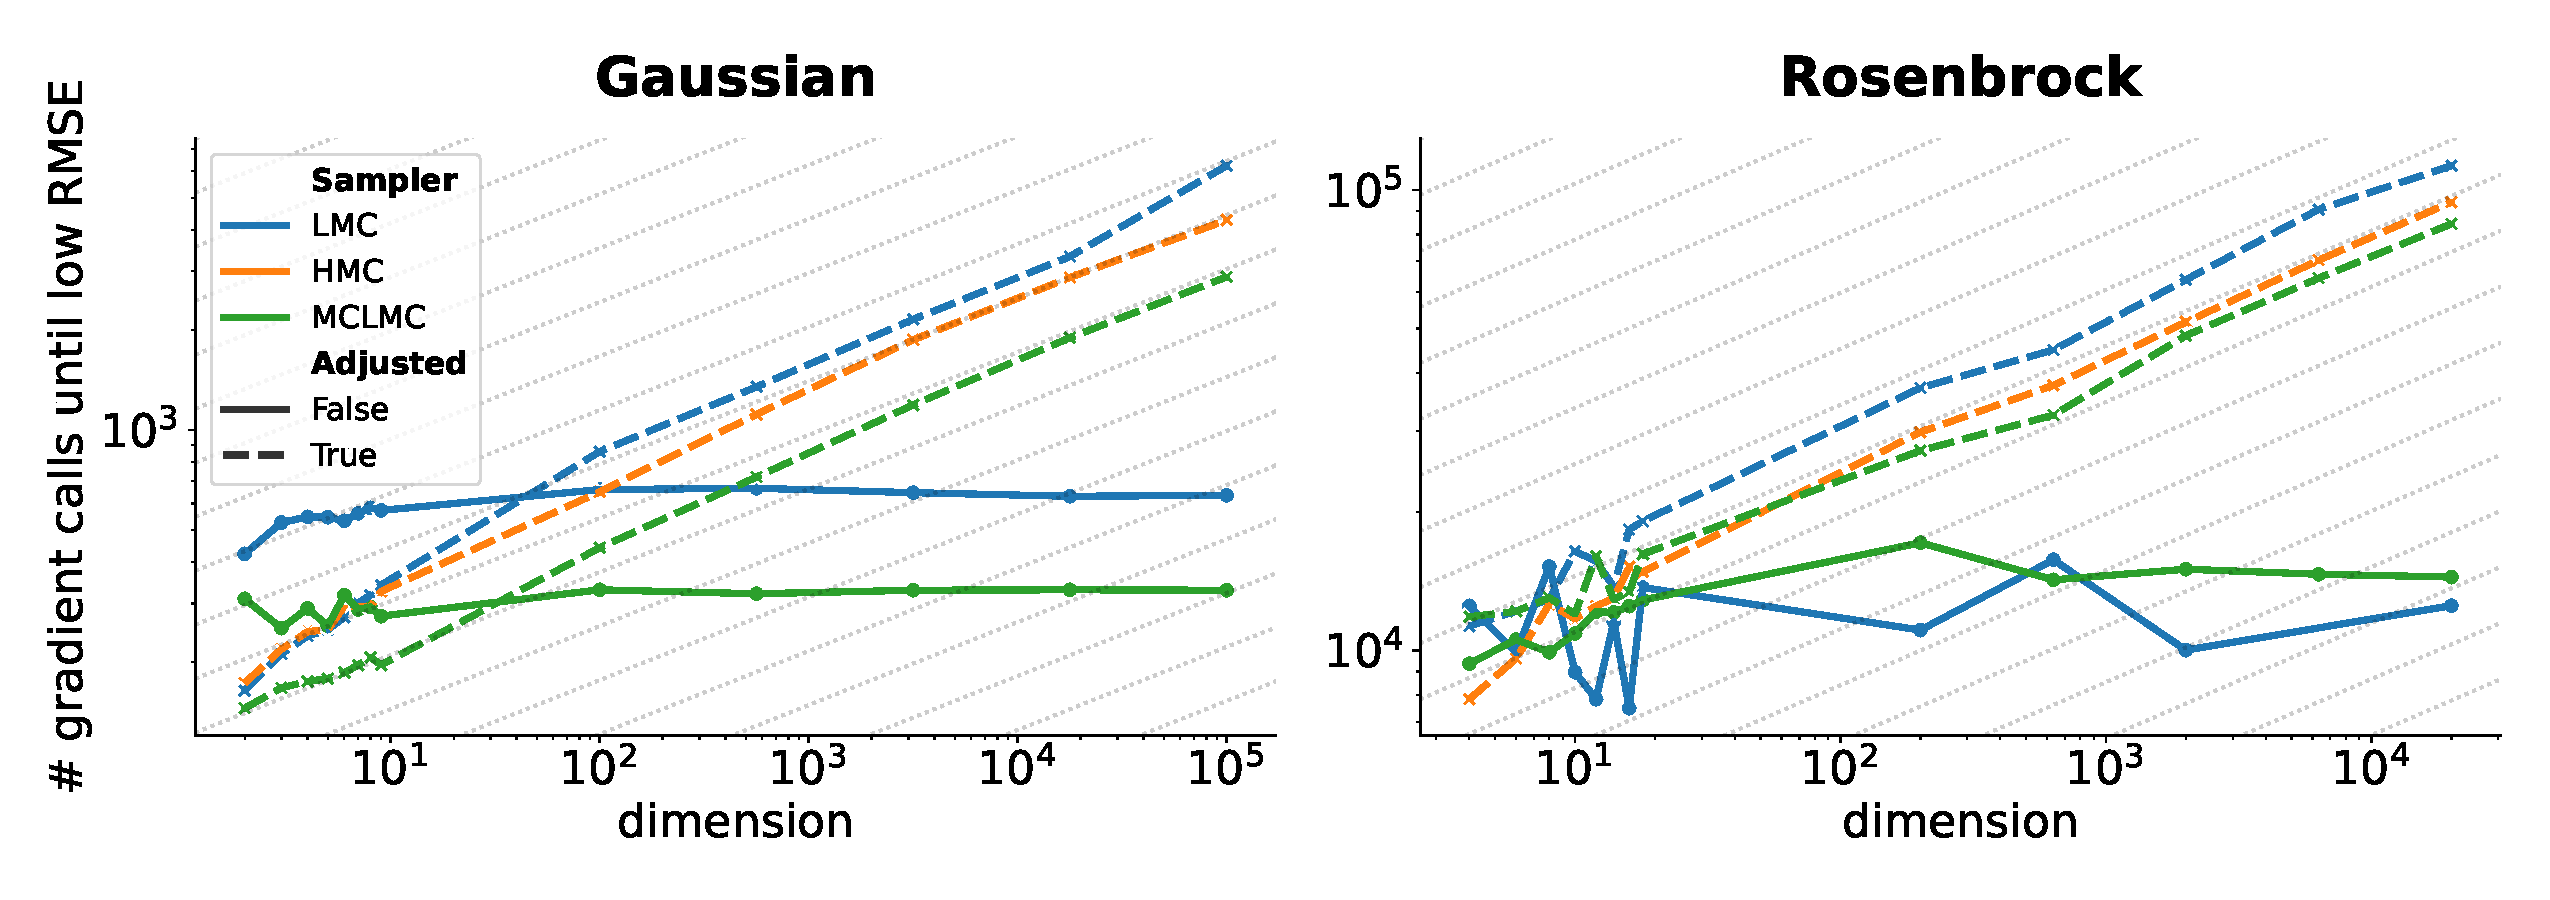
\includegraphics[width=0.95\linewidth]{figures/hmc/scaling.pdf}\\[0.2em]
      {\scriptsize Adjusted cost $\sim d^{1/4}$; unadjusted stays flat.}
    \end{column}
    \begin{column}{0.48\textwidth}
      \centering
      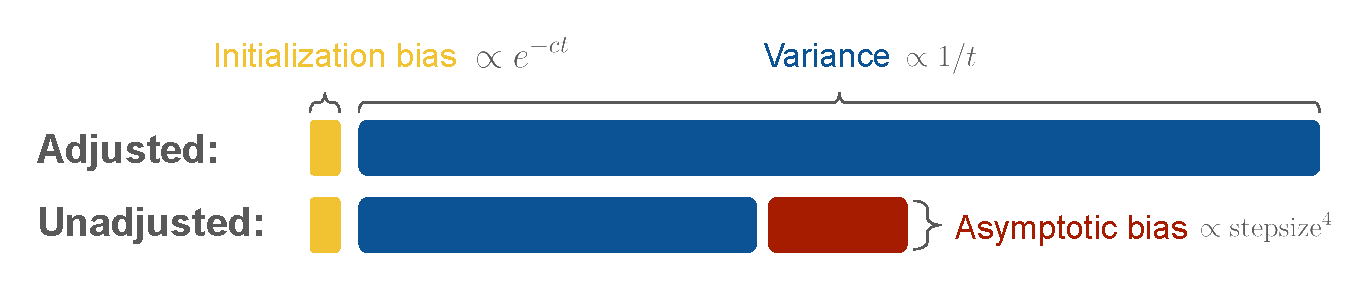
\includegraphics[width=0.95\linewidth]{figures/hmc/bias-variance-diagram.pdf}\\[0.2em]
      {\scriptsize Bias--variance: controlled bias, larger ESS.}
    \end{column}
  \end{columns}
\end{frame}

\begin{frame}{Back to physics: a spin--fermion model}
  Collaboration with \textbf{Peter Lunts} (formerly CCQ):
  unadjusted / microcanonical HMC for a lattice \textbf{spin--fermion} model.

  Two variance sources make this a good stress test:
  \begin{enumerate}\setlength\itemsep{0.35em}
    \item \textbf{Disorder} --- quenched randomness in AFM exchanges.
    \item \textbf{Hutchinson trace trick} --- stochastic traces for fermionic
      observables (noisy gradients / observables).
  \end{enumerate}
  \[
    S[\psi,\bar\psi,n]
    =
    S_{\mathrm{F}}[\psi,\bar\psi]
    +
    S_{\mathrm{b}}[n]
    +
    g\, n\cdot \bar\psi\,\sigma\,\psi
  \]
\end{frame}

\begin{frame}{Results: fermionic observables}
  From \emph{Fast Accurate Quantum Monte Carlo without Metropolis Adjustment}:
  \begin{center}
    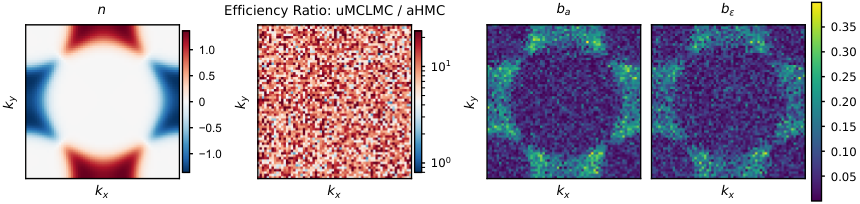
\includegraphics[width=0.95\linewidth]{figures/hmc/results/panel_longrun.png}
  \end{center}
  {\scriptsize $n(\mathbf{k})$; uMCLMC / aHMC efficiency; asymptotic bias $b_a$ and diagnostic $b_\epsilon$.}
\end{frame}

\begin{frame}{Results: efficiency vs~$\lambda$}
  \begin{columns}[T]
    \begin{column}{0.55\textwidth}
      \centering
      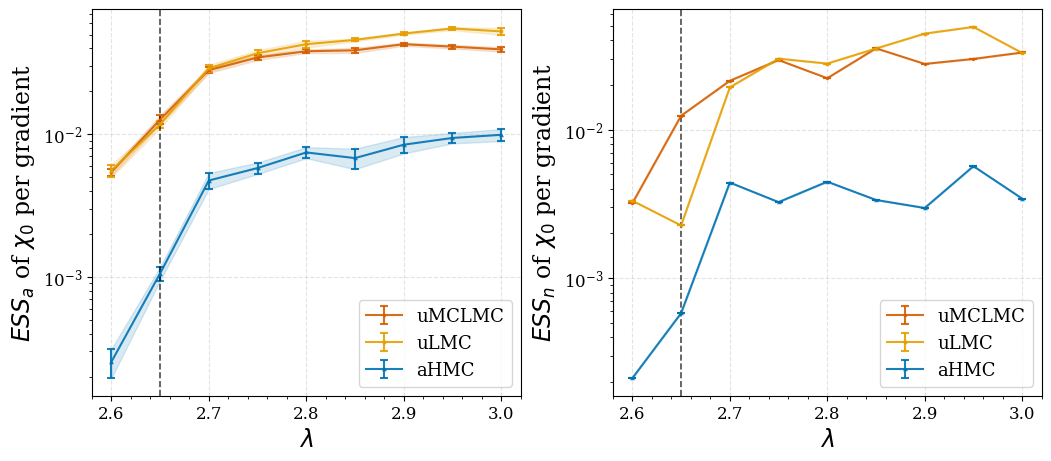
\includegraphics[width=\linewidth]{figures/hmc/results/efficiency_plot.png}
    \end{column}
    \begin{column}{0.42\textwidth}
      \begin{itemize}
        \item Unadjusted \textbf{uMCLMC} / \textbf{uLMC} beat adjusted HMC by roughly an order of magnitude in ESS per gradient
        \item Accuracy matched (bias controlled by step-size tuning)
        \item Gains grow with system size
      \end{itemize}
    \end{column}
  \end{columns}
\end{frame}
